% !TEX root = ../document.tex
\section{Einordnung und Funktionsweise des Image Recognitionings}
\label{sec:Theorie}
Image Recognition (deutsch: Bilderkennung) bezeichnet das Extrahieren, Erkennen und Bezeichnen von bspw. Objekten, Orten, Menschen, Schriften oder Handlungen.\footnote{\cite{ImageRecognition}}  Das, was Menschen schon als Kinder lernen und als selbstverständlich hinnehmen, ist für Computer ein schwer lösbares Problem, dessen Lösung sehr komplexe und rechenintensive Operationen benötigt. Im Gegensatz zu Menschen sieht der Computer ein Bild lediglich als eine Aneinanderreihung von Pixeln bzw. eine Folge von Bits und kann anhand dieser zunächst nichts erkennen.~\footnote{\cite{Tensorflow}}~\footnote{\cite[S.~3]{Burger.2015}} Eine Analyse des Bildes zum Extrahieren sinnvoller Informationen beherrscht ein Computer zunächst nicht.

Ein erster Schritt des Image Recognitionings ist es somit, dem Computer das Erkennen von Merkmalen beizubringen (\textbf{Feature Detection}).~\footnote{\cite[S.~79--80]{Lindeberg.1998}}  Das heißt, ihn anzulernen, anhand der Pixeldaten einfache Merkmale wie z. B. Linien oder Kurven zu erkennen. Dies führt dazu, dass der Computer zwar einfache Merkmale erkennen und extrahieren kann, allerdings besitzt er im Gegensatz zu den Menschen kein weiteres Wissen, es fehlt die Intelligenz. Der Computer muss bei jedem neuen Bild wieder von vorne beginnen („bottom-up“).~\footnote{\cite[S.~3]{Burger.2015}}  Menschen sehen Merkmale und merken sich diese automatisch, sie generieren Wissen. Auch der Computer sollte sich dieses Wissen speichern. Dazu müssen Menschen dem Computer zeigen, wie bestimmte Merkmale aussehen und wie er diese erkennen kann (\textbf{Feature Learning}).~\footnote{\cite[S.~7--8]{HabibiAghdam.2017}}

Nun kann der Computer lediglich die einfachen Merkmale extrahieren, diese allerdings in keinen Kontext setzen und keine komplexeren Muster erkennen. Menschen hingegen besitzen diese Intelligenz bestimmte triviale Merkmale zu Mustern zusammenzusetzen. Dies stellt den nächsten notwendigen Schritt dar: die Mustererkennung (Pattern Recognition). Dies meint, komplexere Merkmale, die sich aus einfachen Merkmalen zusammensetzen, als wiederkehrende Muster in Bildern erkennen zu können. So können zwei horizontale und zwei vertikale Linien (einfache Merkmale), die auf eine bestimmte Weise angeordnet sind, ein Rechteck als Muster ergeben. Ein Muster ist somit eine Menge einfacher Merkmale. Diese Muster können entsprechend der zusammensetzenden Merkmale immer komplexer werden. Für einen Computer würde dies heißen, dass eine bestimmte Anordnung bestimmter Pixel (bzw. eine bestimmte Anordnung von Bits) ein bestimmtes Muster ergeben.~\footnote{\cite[S.~3]{Burger.2015}} Doch selbst wenn der Computer nun Muster erkennen kann, sollte er sich diese auch merken. Menschen erkennen Muster und merken sich diese automatisch, sie speichern diese ab und Generieren somit Wissen. Indem Menschen dem Computer beibringen wie bestimmte Muster in Bildern aussehen und aus welchen Merkmalen sich diese zusammensetzen, kann auch der Computer ein solches Wissen generieren (\textbf{Pattern Classification}).~\footnote{\cite[S.~15--16]{HabibiAghdam.2017}}

Danach muss dem Computer noch beigebracht werden, statt lediglich Muster ganze Objekte in Bildern zu erkennen (\textbf{Object Detection}). Menschen erkennen Objekte anhand verschiedener Muster. Dies muss nun auch der Computer können, das heißt er soll anhand mehrerer zusammengehöriger Muster in einem Bild ein Objekt identifizieren können. Ein Objekt ist somit eine Menge von Mustern. Für einen Computer würde dies heißen, in einem Bild eine bestimmte Anordnung bzw. einen bestimmten Zusammenhang von Mustern (entsprechend von Pixeln bzw. Bits) und anhand dieser somit Objekte zu erkennen.~\footnote{\cite[S.~247--253]{Karray.2017}}  Auch in diesem Falle erkennen Menschen Objekte und merken sich, was diese darstellen. Auch hier muss der Computer ein Wissen entwickeln, das heißt ihm muss von Menschen beigebracht werden, welche Muster sich in welcher Konstellation zu welchem Objekt zusammensetzen (\textbf{Object Classification}).~\footnote{\cite[S.~277]{HabibiAghdam.2017}}

Mit Hilfe dieses Stands können nun mittels Object Detection alle Objekte in einem Bild erkannt und benannt werden. Dahingegen wird beim \textbf{Image Recognition} (auch: \textit{\textbf{Image Classifiation}}) lediglich ein Objekt bzw. eine Klasse in einem Bild erkannt und benannt. Hierbei kann es zwar sein, dass in einem Bild mehrere Objekte bzw. deren Muster erkannt werden, es wird allerdings für jede bekannte Klasse eine Wahrscheinlichkeit berechnet mit der die Klasse in dem Bild vorhanden ist und lediglich die Klasse mit der höchsten Wahrscheinlichkeit wird beim Image Recognitioning benannt (der genaue Prozess wird bei der Erklärung des Covolutional Neural Networks näher erläutert).~\footnote{\cite{SatyaMallick.2016}}~\footnote{\cite{VipulJain.02.04.2018}}

An diesem Stand müssten Menschen die Feature Classification, Pattern Classification und Object Classification allerdings manuell vornehmen, das heißt dem Computer genau beibringen wie (auf Pixelebene bzw. Bitebene) ein Merkmal, ein Muster oder ein Objekt aussieht, was sehr aufwendig wäre. Zudem würde die Erkennung solcher nicht mehr funktionieren, wenn Merkmal, Muster oder Objekt ein wenig von ebenjenem Beigebrachten abweicht. An dieser Stelle spielt das \textbf{Machine Learning} eine Rolle. Mit Hilfe dessen sollen die Classification-Prozesse automatisiert werden. 

Beim maschinellen Lernen wird vor allem zwischen zwei Varianten unterschieden: dem überwachten Lernen (\textbf{supervised learning}) und dem unüberwachten Lernen (\textbf{unsupervised learning}). In beiden Fällen wird dem Computer ein sog. Training Set an Daten (in diesem Falle Bilder von einzelnen Objekten) bereitgestellt. Beim unüberwachten Lernen werden vom Computer eigenständig Muster in den gegebenen Daten erkannt und datenübergreifend verglichen, um Gemeinsamkeiten und Unterschiede in den Daten zu erkennen und diese ggf. gruppieren oder kategorisieren zu können, ohne genau zu wissen, was die Daten darstellen. Bei der Klassifizierung hingegen wird das überwachte Lernen angewendet. Hierbei wird dem Computer für jeden Datensatz mitgeteilt, welche Klasse dieser darstellt (\textbf{Labeling}). Auch hier sollen Objekte und deren Muster und Merkmale erkannt werden, können aber durch das Labeling der jeweiligen Klasse zugeordnet werden, sodass durch das Training Set die Muster und Merkmale der Klassen verfeinert, differenziert und generalisiert werden können. Der Mensch muss dem Computer somit nicht mehr beibringen, wie genau die Muster einer Klasse genau aussehen, sondern der Computer erkennt anhand des Training Sets eigenständig ebensolche und weist sie der Klasse zu. Er erlernt die Muster der gegebenen Klassen selbstständig (Machine Learning).~\footnote{\cite[S.~71--72]{Silva.2016}}

Nun lässt sich Machine Learning allgemein und im Kontext von Image Recognition auch in Beziehung zum Themenbereich \textbf{Big Data} setzen. So profitieren Big Data und Machine Learning jeweils voneinander. So muss auf der einen Seite die stetig wachsende Menge an Daten analysiert werden. Hierbei kann Machine Learning von großem Nutzen sein, da Computer die Daten somit automatisiert analysieren können und durch ihre Analyseverfahren durch das Machine Learning stetig selbstständig verbessern. Auf der anderen Seite werden, wie bereits dargestellt, Training Sets von Daten verwendet, um dem Computer Merkmale und Muster der Klassen anzutrainieren und zu optimieren und so die Analyseverfahren zu verbessern. Je größer dabei die Training Sets sind, desto besser werden diese. Durch die stetig wachsende Menge an Daten stehen dem Computer somit immer mehr Daten für die Training Sets zur Verfügung, sodass die Analyseverfahren stetig besser werden. Konkret für Image Recognition bedeutet dies, dass durch Big Data immer mehr Bildmaterial zur Verfügung steht, anhand dessen die Merkmale und Muster der Klassen und die Analyseverfahren zur Bilderkennung stetig optimiert werden.~\footnote{\cite{MollyGaletto.2018}}~\footnote{\cite{MarcoVarone.}}

\section{TensorFlow als Framework zur maschinellen Bildverarbeitung}
TensorFlow ist ein Open-Source Framework für maschinelles Lernen und soll die Forschung und Entwicklung in diesem Umfeld beschleunigen und verbessern. Mit Hilfe von TensorFlow können im Umfeld von Sprache und Bildverarbeitungsaufgaben neuronale Netze implementiert werden.~\footnote{\cite{OttoGeiler.2018}}~\footnote{\cite{TensorFlow.2018}} Neuronale Netze können in TensorFlow mittels gerichteter zyklenfreier Graphen dargestellt werden. Dabei werden die Inputs und Outputs der einzelnen Rechenschritte durch die Kanten und die Verarbeitung des Inputs zu Output durch die Knoten der Graphen repräsentiert.~\footnote{\cite{OttoGeiler.2018}} TensorFlow findet dabei in vielen Bereichen Anwendung wie z. B. Industrie, Wirtschaft, Finanzen oder Medizin für bspw. Sprachübersetzung oder Früherkennung von Hautkrebs und wird entsprechend auch von vielen großen Unternehmen verwendet wie z. B. SAP, ebay, Twitter oder Nvidia.~\footnote{\cite{TensorFlow.2018}}~\footnote{\cite{OttoGeiler.2018}}

Ein wichtiger Bereich auf den sich TensorFlow konzentriert ist die Bildverarbeitung. TensorFlow teilt diesen wiederum in zwei Sektionen auf: Image Retraining und Image Recognition. Beim Image Retraining geht es vor allem um das Anlernen des Computers. Dazu wird auch bei TensorFlow ein Training Set verwendet, dass Bilder bestimmter Klassen und deren Labels enthält. Diese werden dann von TensorFlow verarbeitet, sodass sich der Computer die Merkmale und Muster der Klassen aneignen kann.~\footnote{\cite{TensorFlow.2017}} Beim Image Recognition geht hingegen darum, zu Erkennen, welche Klasse auf einem Bild, das man dem Computer als Input gibt abgebildet ist.~\footnote{\cite{Tensorflow}} Für das Image Retraining und das Image Recognitioning bietet TensorFlow sowohl eine Python API als auch eine C++ API. Da TensorFlow eine Open Source Library ist, können diese zudem nach Bedarf angepasst werden. Zur direkten praktischen Anwendung des Image Retrainings und Image Recognitionings bietet TensorFlow zudem fertige Skripte an mit Hilfe derer die Software eigens angelernt werden kann oder beim Input eines Bildes die Wahrscheinlichkeit erkannter Klassen ausgibt. Hierzu kann z. B. ein bereits antrainiertes Model heruntergeladen werden oder Training Sets mit vielen Bildern verschiedener Klassen (diese findet man ebenfalls auf der Webseite von TensorFlow). Wie das Image Retraining mit Hilfe der Python API, von TensorFlow zur Verfügung gestellter Skripte und einem eigenen Training Set funktioniert und wie im Anschluss daran Image Recognitioning mit TensorFlow mittels der Python API, von TensorFlow zur Verfügung gestellter Skripte und einem Input-Bild einer antrainierten Klasse betrieben werden kann, wird im praktischen Teil der Ausarbeitung erläutert. Auf der anderen Seite bietet TensorFlow allerdings auch eine Bibliothek mit vielen Funktionen, um in Python oder C++ seine eigenen Skripte zum Image Retraining und Image Recognitioning zu schreiben und so ein eigenes Convolutional Neural Network zu entwickeln.

\section{Convolutional Neural Networks}
TensorFlow arbeitet im Bereich Machine Learning allgemein mit künstlichen neuronalen Netzwerken und im Bereich der Bildverarbeitung konkret mit sog. Convolutional Neural Networks (deutsch: \textit{faltendes neuronale Netzwerke}).~\footnote{\cite{TensorFlow.2018b}}

\subsection{Einordnung}
Der Begriff der neuronalen Netze kommt eigentlich aus der Biologie und beschreibt eine Ansammlung einzelner Neuronen, die eine Netzarchitektur bilden, die aus verschiedenen Schichten besteht. Im Kontext des Machine Learning spricht man allerdings von künstlichen neuronalen Netzen.~\footnote{\cite{JulianMoeser.2017}} Convolutional Neural Networks sind dabei eine spezialisierte Art künstlicher neuronaler Netze. Das Konzept der Convolutional Neural Networks wurde bereits 1989 von LeCun et al. zur Erkennung der menschlichen Handschrift entwickelt.~\footnote{\cite[S.~14]{Christ.2017}}

\subsection{Aufbau und Funktionsweise}
Convolutional Neural Networks bestehen grundsätzlich aus drei verschiedenen Schichten: convolutional layers, pooling layers und fully connected layers. Dabei wird ein Convolutional Neural Network zunächst aus einer Aneinanderreihung von Convolution-Modulen zusammengesetzt. Ein solches Modul besteht dabei jeweils aus einer Convolution Schicht gefolgt von einer Pooling Schicht. Beim Entwickeln eines Convolutional Neural Networks können beliebig viele Convolution-Module aneinandergereiht werden. Auf das letzte Convolution-Modul folgt dann eine oder mehrere Fully Connected Schicht(en).~\footnote{\cite[S.~102]{HabibiAghdam.2017}}~\footnote{\cite{TensorFlow.2018b}} Die folgende Abbildung zeigt ein beispielhaftes Convolutional Neural Network:

\begin{figure}[!h]
	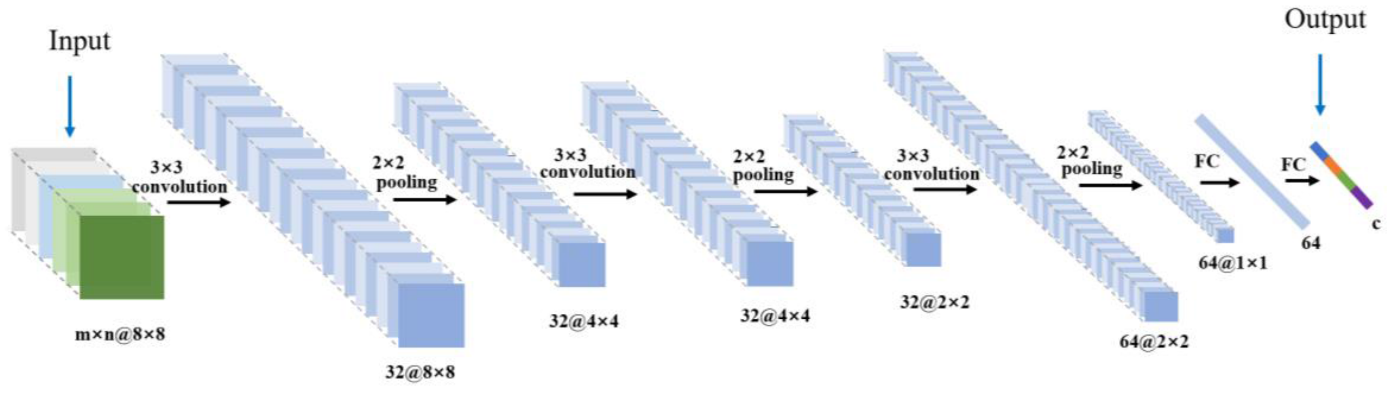
\includegraphics{01.png}
	\caption{Beispielhaftes Convolutional Neural Network. Quelle: \cite[S.~6]{Ji.2018}}
	\label{fig:01}
\end{figure}

Innerhalb der Convolution Schichten findet die Convolution (deutsch: \textit{Faltung}) statt. Input einer Convolution Schicht ist ein Bild. Auf dieses Bild werden dann sog. Filter angewendet.~\footnote{\cite{TensorFlow.2018b}} Filter dienen dazu Merkmale und Muster bzw. Features in dem Eingabebild zu erkennen. Bei der Entwicklung eines Convolutional Neural Networks kann der Entwickler für jede Convolution festlegen, wie viele Filter angewendet werden sollen. Dabei werden verschiedene Filter verwendet, um verschiedene Features zu ermitteln. So kann es bspw. einen Filter zum ermitteln der horizontalen Linien in einem Bild geben. Beim Anwenden eines Filters auf ein Bild wird dabei für jeden Pixel des Eingangsbildes eine vom Filter abhängige mathematische Operation durchgeführt. Für jeden Filter wird dabei ein neues Bild generiert, das heißt, das Eingangsbild wird nicht verändert, sondern das Ergebnis der Berechnung jedes Pixels auf ein neues Bild übertragen, das entsprechend die selbe Größe wie das Eingangsbild besitzt.~\footnote{\cite[S.~90--91]{HabibiAghdam.2017}} Die folgende Abbildung zeigt ein Eingangsbild vor einer Convolution und die durch die Anwendung verschiedener Filter entstandenen Bilder:

\begin{figure}[!h]
	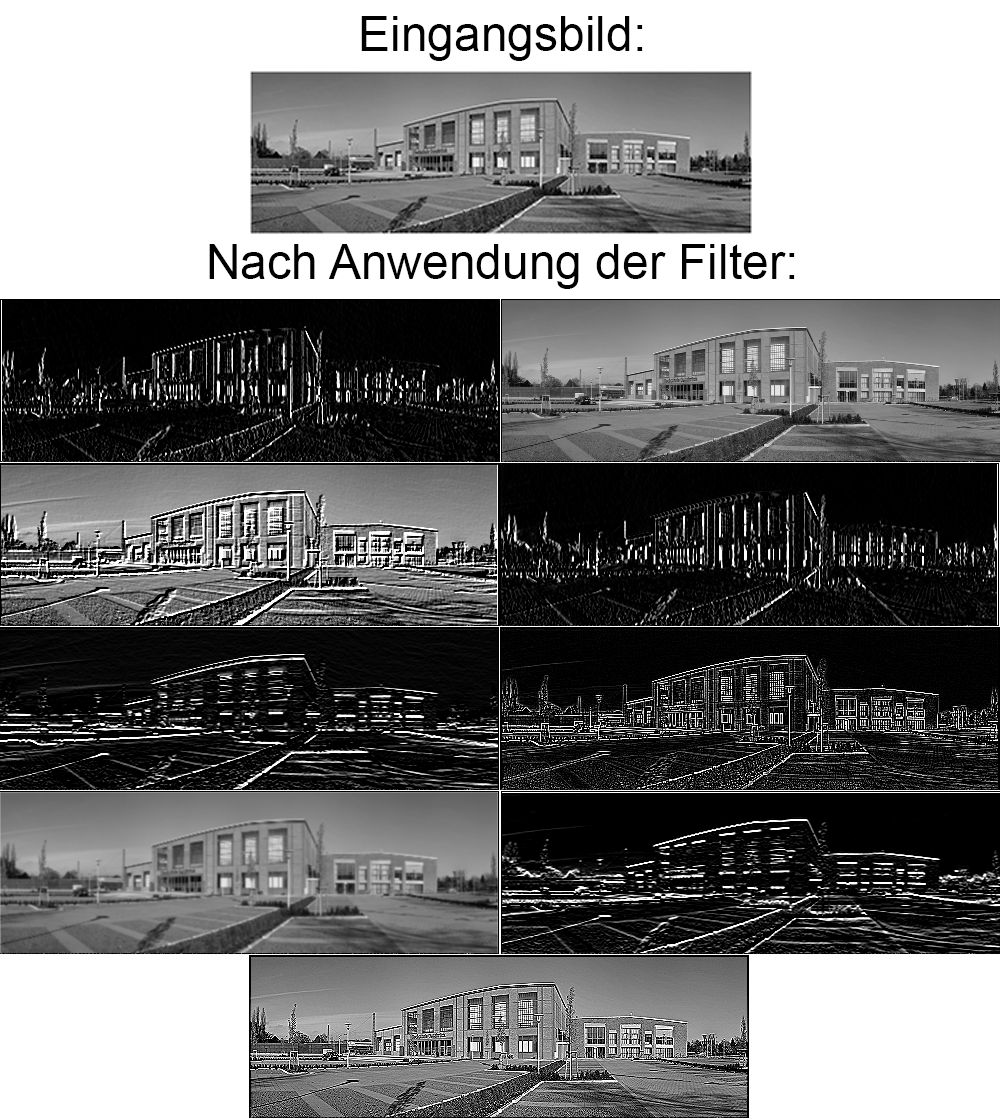
\includegraphics[width=\textwidth]{02.png}
	\caption{Anwendung von Filtern auf ein Bild}
	\label{fig:02}
\end{figure}

Innerhalb der Pooling Schichten findet das Pooling (deutsch: Bündelung) statt. Eine Pooling Schicht folgt auf eine Convolution Schicht und nimmt die Ausgabebilder dieser (nach Anwendung der Filter) als Input. Beim Pooling wird das sog. Downsampling angewendet. Hierbei wird ein bestimmter Pixelbereich der jeweiligen Eingangsbilder zu einem Pixel zusammengefasst und in einem neuen Bild gespeichert. Dadurch soll die Größe der Bilder verringert und sich auf die wesentlichen Merkmale der Bilder beschränkt werden. Es gibt verschiedene Methoden des Poolings, allerdings hat sich herausgestellt, dass das sog. Max-Pooling die besten Ergebnisse liefert. Bei dieser Methode werden z. B. alle Pixel aller Eingangsbilder in 2 x 2 Pixel-Blöcken betrachtet und der Pixel mit dem höchsten Farbwert in das neue, nun kleinere Bild übertragen.~\footnote{\cite{HabibiAghdam.2017}} Die folgende Abbildung zeigt, wie das Max-Pooling aus einem Eingabebild der Größe 32 x 32 Pixel ein Ausgabebild der Größe 16 x 16 Pixel macht:

\begin{figure}[!h]
	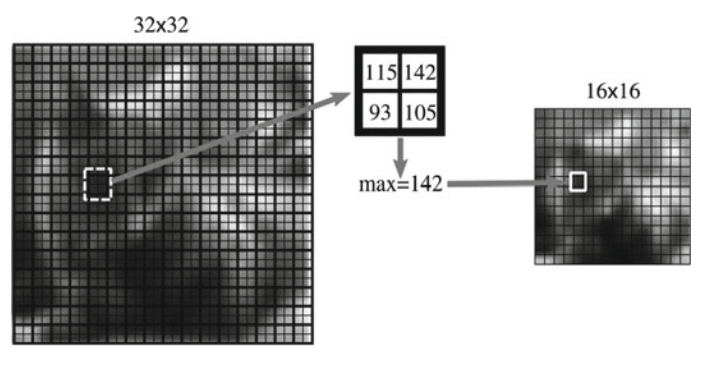
\includegraphics{03.png}
	\caption{Beispiel eines Max-Poolings. Quelle: \cite[S.~96]{HabibiAghdam.2017}}
	\label{fig:03}
\end{figure}

In einer Fully-Connected Schicht werden alle Ausgaben einer Schicht mit allen Ausgaben der nächsten Schicht, das heißt alle erkannten Features einer Schicht mit allen erkannten Features der nächsten Schicht verbunden. Auf diese Weise entstehen kombinierte Features, die für di letztliche Klassifikation von größerer Relevanz sein können.~\footnote{\cite{ujjwalkarn.2016}} Am Ende der letzten Fully-Connected Schicht wird meist die sog. Softmax Funktion angwendet. Diese vergleicht die aus dem Eingangsbild extrahierten Features mit den Features aller bereits bekannten Klassen. Anhand dieses Abgleichs wird dann für jede bereits bekannte Klasse eine Wahrscheinlichkeit berechnet, dass diese in dem Bild abgebildet ist. Die Summe der Wahrscheinlichkeiten aller Klassen ergibt den Wert 1.~\footnote{\cite[S.~14--15]{Brinkmann.2017}}~\footnote{\cite{ujjwalkarn.2016}}~\footnote{\cite{TensorFlow.2018b}}   

Nun kann ein eigenes Convolutional Neural Network entwickelt werden, wobei beliebig viele Schichten hintereinander geordnet werden können. Gibt man nun ein Bild eines Objektes in das Convolutional Neural Network rein, wird eine erste Convolution + Pooling Phase auf dieses angewendet. Der Output dieser Phase dient dann als Input für die nächste Phase. Dies geht solange weiter, bis alle definierten Convolution + Pooling Phasen durchlaufen sind. Dann folgt ein oder mehrere Fully Connected Phasen bis letztlich mittels der Softmax Funktion eine Wahrscheinlichkeit für jede bekannte Klasse errechnet wird. Wie bereits erwähnt, kann bei der Entwicklung eines Convolutional Neural Networks die Anzahl der Filter jeder Convolution ausgewählt werden. Welche Filter letztlich angewendet werden entscheidet dieses allerdings selbst. Anhand der aus den vorherigen Phasen extrahierten Features stellt das Network bereits im Verlauf der Convolution + Pooling Phasen Vermutungen an, was auf dem Bild abgebildet ist und passt die Filter entsprechend dieser Vermutungen an, um so andere bereits gelernte Features durch Filter, die diese abbilden, zu extrahieren.~\footnote{\cite{ujjwalkarn.2016}}~\footnote{\cite[S.~90--91]{HabibiAghdam.2017}} Die Filter werden dabei mit jeder Convolution + Pooling komplexer. So wird anfangs mit einfachen Filtern nach sog. Low-Level Features (z. B. Gerade, Kurven, Ecken, …) und später mit komplexeren Filtern nach High-Level Features (z. B. Gesichter, Hände, …) gesucht.~\footnote{\cite[S.~95]{Takarli.2016}}~\footnote{\cite{ujjwalkarn.2016}} In der folgenden Abbildung ist dargestellt, wie angewendete Filter mit jeder Phase komplexer werden:

\begin{figure}[!h]
	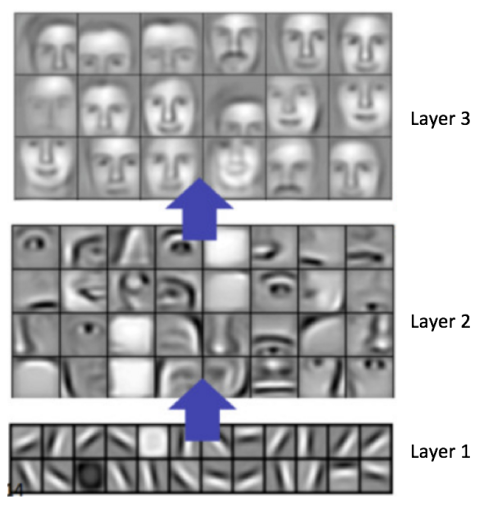
\includegraphics{04.png}
	\caption{Angewendete Filter verschiedener Phasen}
	\label{fig:04}
\end{figure}

\subsection{Image Retraining und Image Recognitioning}
Um das Convolutional Neural Network anzulernen (Image Retraining), wird ein Training Set an Bildern bereitgestellt, wobei dem Network mitgeteilt wird, welche Klassen auf welchem Bild zu sehen ist. Jedes Bild durchläuft dann die vorgesehenen Convolution + Pooling Phasen, in denen das Network mittels ausgewählter Filter die Features aus dem Bild extrahiert und diese erkannten Features der jeweiligen Klasse zuordnet. Je mehr Bilder derselben Klasse das Network verarbeitet, desto feiner und differenzierter werden die Features der Klasse. Durch Bilder anderer Klassen werden die Features zudem von denen anderer Klassen weiter abgegrenzt. Soll nun Image Recognitioning mit dem angelernten Convolutional Neural Network betrieben werden, kann man diesem ein Bild als Input geben, ohne diesem mitzuteilen, was auf diesem Bild abgebildet. Ist mittels der nun bekannten Features der bekannten Klassen werden entsprechende Filter angewendet und entsprechende Features extrahiert. Am Ende werden dann, wie bereits beschrieben, die extrahierten Features mit denen der bekannten Klassen verglichen und für jede Klasse eine Wahrscheinlichkeit berechnet.